\documentclass[norsk, 11pt]{article}

\usepackage{booktabs}       % Ordentlige tabeller
\usepackage{url}            % Skrive url-er
\usepackage{textcomp}       % Den greske bokstaven micro i text-mode
\usepackage{units}          % Skrive enheter riktig
\usepackage{float}          % Figurer dukker opp der du ber om
\usepackage{listingsutf8}   % Kodetekst
\usepackage{subfigure}		% Flere fig. ved siden av hverandre
\usepackage{obligJV}


\lstset{breaklines=True,numbers=left}

% JF i margen
\makeatletter
\renewcommand{\subsubsection}{\@startsection{subsubsection}{3}{-2cm}%
{-\baselineskip}{0.5\baselineskip}{\bf\large}}
\makeatother
\newcommand{\jf}[1]{\subsubsection*{JF #1}\vspace*{-2\baselineskip}}

% Skru av seksjonsnummerering
\setcounter{secnumdepth}{-1}

%, trim = 1cm 7cm 1cm 7cm % PDF-filer som bilde

\begin{document}

% Forside
\begin{titlepage}
\begin{center}

\textsc{\Large FYS4150 - Computational Physics}\\[0.5cm]
\rule{\linewidth}{0.5mm} \\[0.4cm]
{ \huge \bfseries  PROSJEKT 2}\\[0.10cm]
\rule{\linewidth}{0.5mm} \\[1.5cm]
\textsc{\Large Å løse Schrödingers likning for étt og to elektroner}\\[1.5cm]
\textsc{}\\[1.5cm]

% Av hvem?

\begin{minipage}{0.49\textwidth}
    \begin{center} \large
        Jon Vegard Sparre\\ \url{jonvsp@uio.no} \\[0.8cm]
    \end{center}
\end{minipage}


\vfill

% Dato nederst
\large{Dato: \today}

\end{center}
\end{titlepage}

\abstract{I dette prosjektet har vi løst Schrödingerlikninga for harmonisk oscillator med ett og to elektroner. Vi har brukt Jacobis metode og egenverdi-løseren til Armadillo-biblioteket for å løse den numerisk. De numeriske resultatene har blitt sammenliknet med de analytiske resultatene til M. Taut (sett inn ref. her) Vi har kun sett på løsningene for relativ avstand med og uten Coulomb-frastøtning.}

Lenke til mitt GitHub domene: \url{https://github.com/jonvegards/FYS4150}

\subsection*{Introduksjon}
Problemet som vi kommer til å løse i dette prosjektet er Schrödingerlikninga (SL) for en 3D harmonisk oscillator med ett og to elektroner. Vi har et sfærisk symmetrisk potensiale, som gjør at vi trenger kun å løse den radielle SL, \emph{i.e.} vi har redusert det tredimensjonale problemet til et éndimensjonalt ett. Den radielle delen av SL er da, for en harmonisk oscillator
$$ -\frac{\hbar^2}{2m} \para{ \frac{1}{r^2} \frac{\dd}{\dr}r^2 \frac{\dd}{\dr} - \frac{l(l+1)}{r^2}}R(r) + \frac{m\omega^2r^2}{2} R(r) = E R(r).$$
Det er essensielt denne likninga vi skal løse gjennom hele prosjeket i forskjellige former. Metoden vi skal bruke her, ble vi kjent med i prosjekt 1. Vi tar utgangspunkt i trepunktsformelen for en annenderivert, diskretiserer funksjonen i $n$ steg med en steglengde $h$, setter det opp som en tridiagonal matrise og løser matriselikninga med en egnet algoritme.

\subsection*{Teori}
SL er gitt i sfæriske koordinater, s.a. $r\in [0,\infty)$. Denne likninga inneholder noen stygge annenderiverte som vi vil endre på, så vi substituerer $R(r) = (1/r)u(r)$ og får,
$$ -\frac{\hbar^2}{2m}\frac{\dd^2}{\dr^2}u(r) + \para{\frac{\hbar^2}{2m}\frac{l(l+1)}{r^2} + \frac{m\omega^2r^2}{2}} u(r) = E u(r).$$
Randbetingelsene her er greie å finne ut av, vi vet at $u(0) = 0$ og at $u(\infty) = 0$ siden 

Prøver vi å putte likninga inn i et program slik den er nå, så vil vi få noen ubehagelige overraskelser hva gjelder avrundingsfeil, overflow og andre ting vi ikke vil ha i en numerisk løsning. Vi innfører derfor dimensjonsløse variable, da blir resultatet automagisk på den lengdeskalaen problemet krever at det er. Først setter vi $ \rho = (1/ \alpha)r$, $\alpha$ er en konstant med dimensjon lengde. Ved å sette inn dette får vi
$$ -\frac{\hbar^2}{2m\alpha^2}\frac{\dd^2}{\dd\rho^2}u(\rho) + \para{\frac{\hbar^2}{2m\alpha^2}\frac{l(l+1)}{r^2} + \frac{m\omega^2\alpha^2\rho^2}{2}} u(\rho) = E u(\rho), $$
vi vil ha den annenderiverte for seg selv, så vi ganger med $2m\alpha^2/\hbar^2$ på begge sider og får
$$ -\frac{\dd^2}{\dd\rho^2}u(\rho) + \para{\frac{l(l+1)}{r^2} + \frac{m^2\omega^2\alpha^4\rho^2}{\hbar^2}} u(\rho) = \frac{2m\alpha^2}{\hbar^2}E u(\rho), $$
en siste endring vi gjør er å sette $m^2\omega^2\alpha^4/\hbar^2=1$ og vi introduserer $ \lambda = 2m\alpha^2 E/ \hbar^2$. Vi skal i dette prosjektet kun se på løsninger med $l=0$, alt dette gir oss da likninga vi skal implementere i programmet,
$$ -\frac{\dd^2}{\dd\rho^2}u(\rho) + \rho^2u(\rho) = \lambda u(\rho). $$
Den analytiske løsninga for dette problemet gir oss egenverdiene $\lambda_1 = 3$, $\lambda_2 = 7$ og $\lambda_3 = 11$.

Det er ingen grunn til å vente med å se på likninga for problemet med to elektroner, så vi gyver løs på den med en gang. Vi vil så gå gjennom hvordan vi diskretiserer likninga og får den på matriseform, slik vi gjorde i prosjekt 1. For et system med to elektroner vil SL (uten Coulombinteraksjoner) være
$$ \para{- \frac{ \hbar^2}{2m} \frac{\dd^2}{\dr_1^2} - \frac{ \hbar^2}{2m} \frac{\dd^2}{\dr_2^2} + \frac{1}2 k_1r_1^2 + \frac{1}2 k_2r_2^2} u(r_1,r_2) = E^{(2)}u(r_1,r_2), $$
hvor $r_1$ og $r_2$ er posisjonene til elektron 1 og elektron 2, energien $E^{(2)}$ er den samla energien til systemet og $k_i = m\omega_i^2$. Vi introduserer så den relativet koordinaten $r = r_1 - r_2$ og massesenterkoordinaten $R = (1/2)(r_1 + r_2)$, SL tar da formen
$$ \para{- \frac{ \hbar^2}{m} \frac{\dd^2}{\dr^2} - \frac{ \hbar^2}{4m} \frac{\dd^2}{\dd R^2} + \frac{1}4 m\omega_r^2r^2 + m\omega_R^2R^2} u(r,R) = E^{(2)}u(r,R). $$
Dette er heldigvis en separabel differensiallikning, så vi kan sette $u(r,R) = \psi(r)\phi(R)$ og bruke at energien er gitt som $E^{(2)} = E_r + E_R$. Vi legger også til Coulombinteraksjonen, som avhenger av avstanden mellom elektronene,
$$ V(r) = \frac{\beta e^2}r. $$ 
Vi får da
$$ \para{- \frac{ \hbar^2}{m} \frac{\dd^2}{\dr^2} + \frac{1}4 m\omega_r^2r^2 + \frac{\beta e^2}r} \psi(r) = E_r\psi(r). $$
Vi gjentar substitusjonsprosessen som vi gjorde over, $r = (1/\alpha)$. Vi setter $\alpha  = \hbar / m\beta e^2$, $\omega_r^2 = (1/4)(mk\alpha^4/\hbar^2)$ og definerer $ \lambda = m \alpha^2 E/\hbar$, dette gir oss
$$ - \frac{\dd^2}{\dd \rho^2} \psi(\rho) + \omega_r^2\rho^2 + \frac{1}\rho  \psi(\rho) = \lambda \psi(\rho). $$
Vi ser at eneste forskjellen fra i stad er at vi har fått et ekstra potensialledd, hvilket betyr at vi kan lage én algoritme som løser for begge tilfellene.

\subsection*{Metode}
Nå som vi har stablet på beina likningen vi skal løse, så kan vi ta en titt på den numeriske delen. Vi skal bruke trepunktsformelen for en annenderivert, som vi her kan skrive som
$$ u'' = \frac{u(\rho + h) - 2u(\rho) + u(\rho - h)}{h^2} + \mathcal{O}(h^2) $$

\subsection*{Resultater}

\subsection*{Konklusjon}



\end{document}

\begin{align*}
	Av &=
	\left(\begin{matrix}
		2 & -1 & 0 & 0 &\ldots & 0 \\	
		-1 & 2 & -1 & 0 & \ldots & 0 \\
		0 & \ddots & \ddots & \ddots & \ddots & \vdots \\
		\vdots & \ddots & \ddots & \ddots & \ddots & 0 \\
		\vdots & \ddots & \ddots & \ddots & \ddots & -1 \\
		0 & \ldots & \ldots & 0 & -1 & 2 \\
	\end{matrix}\right)\left(
	\begin{matrix}
		v_1 \\ \vdots\\ \vdots \\ \vdots \\ v_n 
	\end{matrix} \right) \\
	&= \left(\begin{matrix}
		2v_1 & -v_2 & 0 & 0 &\ldots & 0 \\	
		-v_1 & 2v_2 & -v_3 & 0 & \ldots & 0 \\
		0 & \ddots & \ddots & \ddots & \ddots & \vdots \\
		\vdots & \ddots & \ddots & \ddots & \ddots & 0 \\
		\vdots & \ddots & \ddots & \ddots & \ddots & -v_n \\
		0 & \ldots & \ldots & 0 & -v_{n-1} & 2v_n \\
	\end{matrix}\right),
\end{align*}

\begin{table}[H]
  \centering
  \begin{tabular}{ c c }
    \toprule
    $n$ & $\epsilon_{\text max}$ \\
    \midrule
	$10$ &	$-1.1797$ \\
	$10^2$ & $-3.0880$ \\
	$10^3$ & $-5.0800$ \\
	$10^4$ & $-7.0753$ \\
	$10^5$ & $-8.3667$ \\
    \bottomrule
  \end{tabular}
  \caption{Maximum error for different $n$ when using LU-decomposition with forward and backward substitution. At $n=10^6$ our program crashes. Also note that the error is decreasing with increasing $n$.}
  \label{tab:error_max}
\end{table}

%\begin{figure}[H]
%    \centering
%    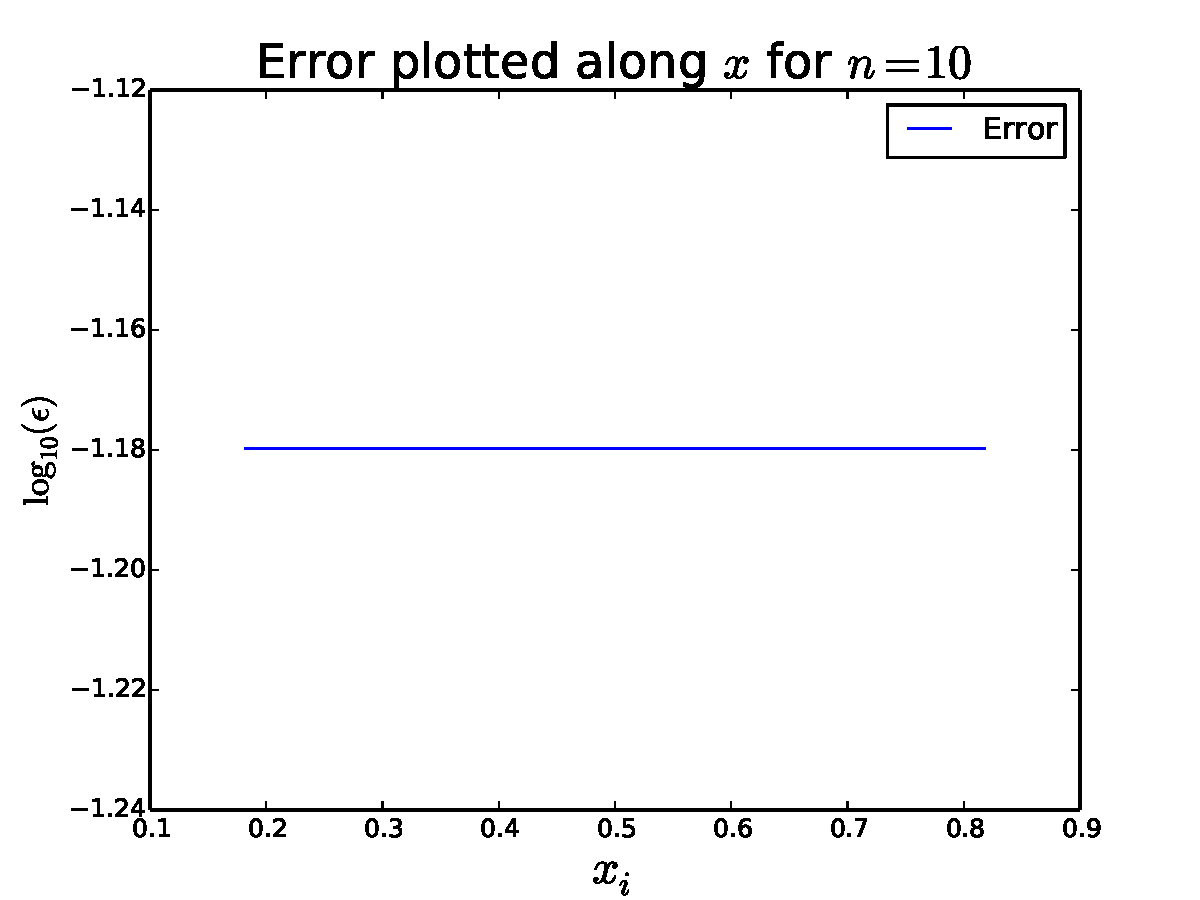
\includegraphics[width = .9\textwidth]{error_n_10.pdf}
%    \caption{When $n=10$ the error is constant, this may be a coincidence. The error is quite big anyway, which we also see clearly in fig. \ref{fig:sol101}.}
%    \label{fig:en101}
%\end{figure}
